\documentclass[12pt]{article}
\usepackage[utf8]{inputenc}
\usepackage{geometry}
\usepackage{hyperref}
\usepackage{graphicx}
\usepackage{tabularx}
\usepackage{enumitem}
\geometry{a4paper, margin=1in}
\title{\textbf{Settlers of Catan - Strategy Guide}}
\author{Miguel Cabral Pinto}
\date{}

\begin{document}
\maketitle
\renewcommand{\contentsname}{Contents}
\tableofcontents
\newpage

\section{Introduction}
I made this guide to share my understanding of the board game Settlers of Catan\texttrademark\space with my friends.
It serves as a compendium of information I gathered from other strategy guides mixed with my own knowledge, so it is recommended to have some notion of the game rules before reading, which can be found \href{https://colonist.io/catan-rules}{here}.
Finally, this document is meant to be improved over time, so feel free to give me any kind of suggestions!

\section{Fundamentals}

\subsection{Resources}
\begin{tabularx}{\textwidth}{|p{0.14\textwidth}|p{0.08\textwidth}|X|p{0.08\textwidth}|}
    \hline
    \textbf{Resource} & \textbf{Use} & \textbf{Value} & \textbf{Hexes} \\
    \hline
    \raisebox{-0.5\height}{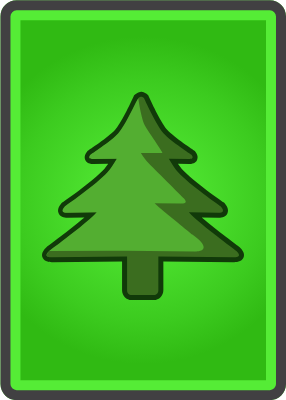
\includegraphics[height=10pt]{../imgs/wood.png} \textbf{Wood}} & \raisebox{-0.5\height}{
\includegraphics[height=10pt]{../imgs/settle.png} 
\includegraphics[height=10pt]{../imgs/road.png}} & Extra value at the start of the game, and for Longest Road strategies. & 4 \\
    \hline
    \raisebox{-0.5\height}{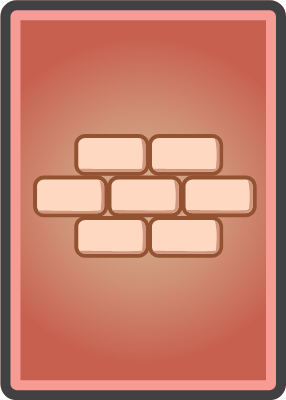
\includegraphics[height=10pt]{../imgs/brick.png} \textbf{Brick}} & \raisebox{-0.5\height}{
\includegraphics[height=10pt]{../imgs/settle.png} 
\includegraphics[height=10pt]{../imgs/road.png}} & Like \raisebox{-0.15\height}{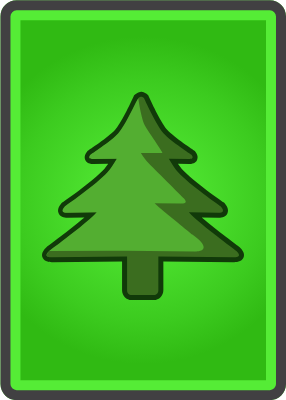
\includegraphics[height=10pt]{../imgs/wood.png}}, but scarcer, so it generally becomes more valuable. & 3 \\
    \hline
    \raisebox{-0.5\height}{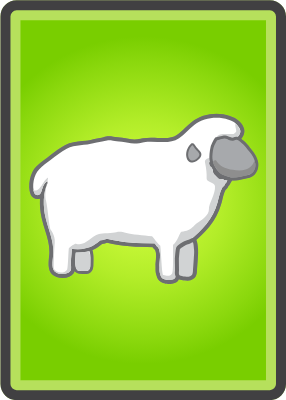
\includegraphics[height=10pt]{../imgs/sheep.png} \textbf{Sheep}} & \raisebox{-0.5\height}{
\includegraphics[height=10pt]{../imgs/settle.png} 
\includegraphics[height=10pt]{../imgs/dev.png}} & Moderate value, but always needed for any strategy, especially if buying \raisebox{-0.15\height}{
\includegraphics[height=10pt]{../imgs/dev.png}}. & 4 \\
    \hline
    \raisebox{-0.5\height}{
\includegraphics[height=10pt]{../imgs/wheat.png} \textbf{Wheat}} & \raisebox{-0.5\height}{
\includegraphics[height=10pt]{../imgs/settle.png} 
\includegraphics[height=10pt]{../imgs/city.png} 
\includegraphics[height=10pt]{../imgs/dev.png}} & Very valuable throughout the game, as it is needed for almost everything. & 4 \\
    \hline
    \raisebox{-0.5\height}{
\includegraphics[height=10pt]{../imgs/ore.png} \textbf{Ore}} & \raisebox{-0.5\height}{
\includegraphics[height=10pt]{../imgs/city.png} 
\includegraphics[height=10pt]{../imgs/dev.png}} & Very valuable, especially in the late game, where \raisebox{-0.1\height}{
\includegraphics[height=10pt]{../imgs/city.png}} are the best way to increase production. & 3 \\
    \hline
\end{tabularx}

\subsection{Purchases}
\begin{tabularx}{\textwidth}{|p{0.15\textwidth}|p{0.12\textwidth}|X|p{0.07\textwidth}|}
    \hline
    \textbf{Purchase} & \textbf{Cost} & \textbf{Benefit} & \textbf{VPs} \\
    \hline
    \raisebox{-0.5\height}{
\includegraphics[height=10pt]{../imgs/road.png} \textbf{Road}} & \raisebox{-0.5\height}{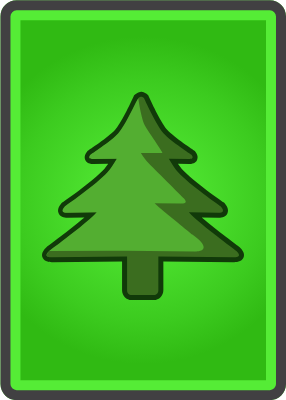
\includegraphics[height=10pt]{../imgs/wood.png} 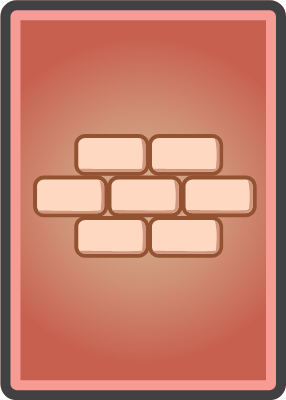
\includegraphics[height=10pt]{../imgs/brick.png}} & Expands the network of placeable \raisebox{-0.1\height}{
\includegraphics[height=10pt]{../imgs/settle.png}} and can contribute to Longest Road. & 0 \\
    \hline
    \raisebox{-0.5\height}{
\includegraphics[height=10pt]{../imgs/settle.png} \textbf{Settlement}} & \raisebox{-0.5\height}{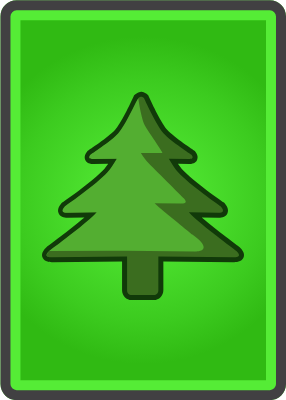
\includegraphics[height=10pt]{../imgs/wood.png} 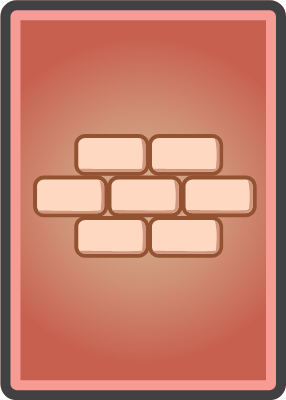
\includegraphics[height=10pt]{../imgs/brick.png} 
\includegraphics[height=10pt]{../imgs/wheat.png} 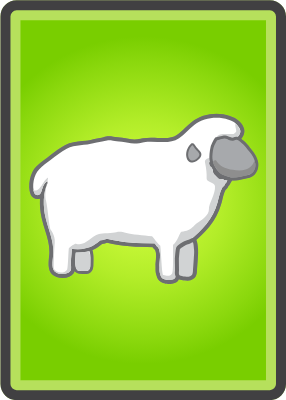
\includegraphics[height=10pt]{../imgs/sheep.png}} & Grants resources to the player if the number of adjacent hexes is rolled. Most common way to increase production early, to claim as much space as possible. Must be 2 spaces away from other \raisebox{-0.1\height}{
\includegraphics[height=10pt]{../imgs/settle.png}}. & 1 \\
    \hline
    \raisebox{-0.5\height}{
\includegraphics[height=10pt]{../imgs/city.png} \textbf{City}} & \raisebox{-0.5\height}{
\includegraphics[height=10pt]{../imgs/ore.png} 
\includegraphics[height=10pt]{../imgs/ore.png} 
\includegraphics[height=10pt]{../imgs/ore.png} 
\includegraphics[height=10pt]{../imgs/wheat.png} 
\includegraphics[height=10pt]{../imgs/wheat.png}} & Doubles the resource production of a \raisebox{-0.1\height}{
\includegraphics[height=10pt]{../imgs/settle.png}}. In the late game, it's the only way to improve production, but if built early it can be very strong. & 2 \\
    \hline
    \raisebox{-0.5\height}{
\includegraphics[height=10pt]{../imgs/dev.png} \textbf{Dev Card}} & \raisebox{-0.5\height}{
\includegraphics[height=10pt]{../imgs/ore.png} 
\includegraphics[height=10pt]{../imgs/wheat.png} 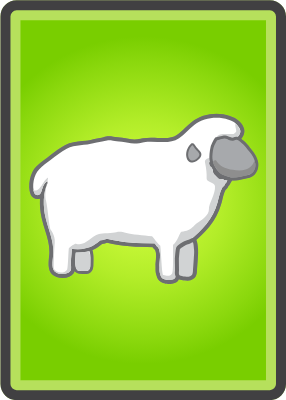
\includegraphics[height=10pt]{../imgs/sheep.png}} & Mystery card that can contribute to both achievements and contain VPs and useful abilities. & Var. \\
    \hline
\end{tabularx}

% \subsection{Achievements}
% \begin{tabularx}{\textwidth}{|p{0.21\textwidth}|X|}
%     \hline
%     \textbf{Achievement} & \textbf{Description} \\
%     \hline
%     \raisebox{-0.5\height}{\raisebox{-0.15\height}{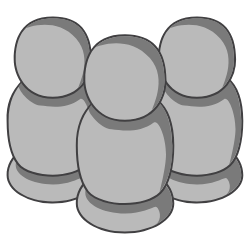
\includegraphics[height=10pt]{../imgs/army.png}} \textbf{Largest Army}} & The first player to reach the current maximum number of used \raisebox{-0.15\height}{
\includegraphics[height=10pt]{../imgs/knight.png}} above 3 gets 2 VPs.\\
%     \hline
%     \raisebox{-0.5\height}{\raisebox{-0.15\height}{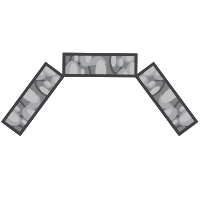
\includegraphics[height=10pt]{../imgs/longest_road.png}} \textbf{Longest Road}} & The first player to have the current longest sequence of consecutive \raisebox{-0.15\height}{
\includegraphics[height=10pt]{../imgs/road.png}} above 5 gets 2 VPs.\\
%     \hline
% \end{tabularx}

\subsection{Development Cards}
\begin{tabularx}{\textwidth}{|p{0.16\textwidth}|X|}
    \hline
    \textbf{Card} & \textbf{Benefit} \\
    \hline
    \raisebox{-0.5\height}{
\includegraphics[height=10pt]{../imgs/knight.png} \textbf{Knight}} & When played, allows the user to move the Robber and steal a random card from a blocked player. Uses include removing the Robber from a key hex, slowing opponents by blocking them, and contributing to Largest Army. \\
    \hline
    \raisebox{-0.5\height}{
\includegraphics[height=10pt]{../imgs/vp.png} \textbf{VP}} & When bought, gives the owner a hidden VP. Its possession should be kept secret as long as possible, so the player's real score remains a mystery to others. \\
    \hline
    \raisebox{-0.5\height}{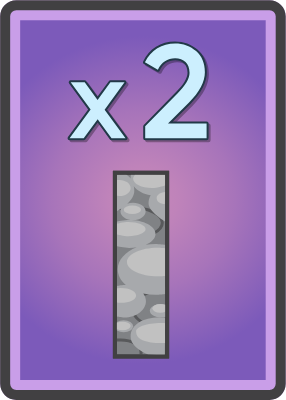
\includegraphics[height=10pt]{../imgs/road_building.png} \textbf{Road}} \newline \raisebox{-0.5\height}{\textbf{Building}} & When played, the user may build 2 \raisebox{-0.15\height}{
\includegraphics[height=10pt]{../imgs/road.png}} connected to their network. Very useful early to move around the board without spending \raisebox{-0.15\height}{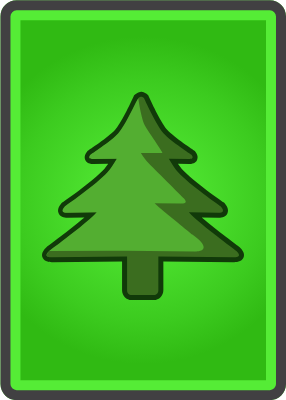
\includegraphics[height=10pt]{../imgs/wood.png} 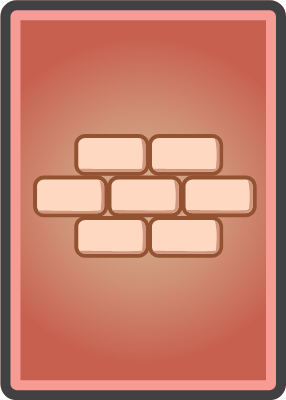
\includegraphics[height=10pt]{../imgs/brick.png}}, making it easier to establish \raisebox{-0.1\height}{\includegraphics[height=10pt]{../imgs/settle.png}}. Also contributes to Longest Road.\\
    \hline
    \raisebox{-0.5\height}{\includegraphics[height=10pt]{../imgs/yop.png} \textbf{Year}} \newline \raisebox{-0.5\height}{\textbf{of Plenty}} & When played, the user chooses 2 resource cards from the bank. Should be used to get unproduced resources or to finish a project missing cards. (Ex: \raisebox{-0.15\height}{\includegraphics[height=10pt]{../imgs/wheat.png} \includegraphics[height=10pt]{../imgs/wheat.png} \includegraphics[height=10pt]{../imgs/ore.png}} + (\raisebox{-0.15\height}{\includegraphics[height=10pt]{../imgs/yop.png}} $\rightarrow$ \raisebox{-0.15\height}{\includegraphics[height=10pt]{../imgs/ore.png} \includegraphics[height=10pt]{../imgs/ore.png}}) = \raisebox{-0.1\height}{\includegraphics[height=10pt]{../imgs/city.png}})\\
    \hline
    \raisebox{-0.5\height}{\includegraphics[height=10pt]{../imgs/mono.png} \textbf{Monopoly}} & When played, the user takes all cards of a specific resource from other players' hands. Considered very strong for its potential to control the supply of a resource and excellent synergy with ports. \textit{``You should always try to get at least 2 points from a \raisebox{-0.15\height}{\includegraphics[height=10pt]{../imgs/mono.png}}!''} - DandyDrew (Catan King)\\
    \hline
\end{tabularx}

\section{Strategies}

\begin{itemize}
    \item \textbf{OWS $\rightarrow$}
    Starting resources: \raisebox{-0.15\height}{\includegraphics[height=10pt]{../imgs/sheep.png} \includegraphics[height=10pt]{../imgs/wheat.png} \includegraphics[height=10pt]{../imgs/ore.png}}.
    Focus on Largest Army.
    The chosen resources allow quick investment in \raisebox{-0.1\height}{\includegraphics[height=10pt]{../imgs/city.png}} and \raisebox{-0.15\height}{\includegraphics[height=10pt]{../imgs/dev.png}}, depending on trades with the bank and/or other players to get the necessary \raisebox{-0.15\height}{\includegraphics[height=10pt]{../imgs/wood.png} \includegraphics[height=10pt]{../imgs/brick.png}} for minimal mobility.
    After overcoming this difficulty and building a \raisebox{-0.1\height}{\includegraphics[height=10pt]{../imgs/settle.png}}, it can be very strong, as it allows the hardest objectives to be advanced early.
    \item \textbf{Hybrid OWS $\rightarrow$}
    Starting resources: \raisebox{-0.15\height}{\includegraphics[height=10pt]{../imgs/sheep.png} \includegraphics[height=10pt]{../imgs/wheat.png} \includegraphics[height=10pt]{../imgs/ore.png}} (\raisebox{-0.15\height}{\includegraphics[height=10pt]{../imgs/wood.png}} \raisebox{-0.15\height}{\includegraphics[height=10pt]{../imgs/brick.png}}).
    Focus on Largest Army.
    Combines the previous strategy with \raisebox{-0.15\height}{\includegraphics[height=10pt]{../imgs/wood.png}} or \raisebox{-0.15\height}{\includegraphics[height=10pt]{../imgs/brick.png}}, trading some OWS resource production for flexibility.
    In most cases, pure OWS is unviable due to the scarcity of good starting spots, so this is the closest possible.
    \item \textbf{Road $\rightarrow$}
    Starting resources: \raisebox{-0.15\height}{\includegraphics[height=10pt]{../imgs/wood.png} \includegraphics[height=10pt]{../imgs/brick.png}} (\raisebox{-0.15\height}{\includegraphics[height=10pt]{../imgs/sheep.png} \includegraphics[height=10pt]{../imgs/wheat.png} \includegraphics[height=10pt]{../imgs/ore.png}}).
    Focus on Longest Road.
    Prioritizes rapid expansion early, as controlling a portion of the board greatly helps this strategy, and allows building \raisebox{-0.1\height}{\includegraphics[height=10pt]{../imgs/settle.png}}.
    \item \textbf{City + Road $\rightarrow$}
    Starting resources: \raisebox{-0.15\height}{\includegraphics[height=10pt]{../imgs/wood.png} \includegraphics[height=10pt]{../imgs/brick.png} \includegraphics[height=10pt]{../imgs/wheat.png} \includegraphics[height=10pt]{../imgs/ore.png}}.
    Focus on Longest Road.
    Compared to \textbf{Road}, balances the initial investment to allow building a \raisebox{-0.1\height}{\includegraphics[height=10pt]{../imgs/city.png}}, being very flexible by having another way to score points and increase production.
    \item \textbf{5 Resources $\rightarrow$}
    Starting resources: \raisebox{-0.15\height}{\includegraphics[height=10pt]{../imgs/wood.png} \includegraphics[height=10pt]{../imgs/brick.png} \includegraphics[height=10pt]{../imgs/sheep.png} \includegraphics[height=10pt]{../imgs/wheat.png} \includegraphics[height=10pt]{../imgs/ore.png}}.
    General focus.
    Max flexibility!
    \item \textbf{Port $\rightarrow$}
    Starting resources: (\raisebox{-0.15\height}{\includegraphics[height=10pt]{../imgs/wood.png} \includegraphics[height=10pt]{../imgs/brick.png} \includegraphics[height=10pt]{../imgs/sheep.png} \includegraphics[height=10pt]{../imgs/wheat.png} \includegraphics[height=10pt]{../imgs/ore.png}}).
    General focus.
    Happens when you have access to a lot of a specific resource and the corresponding 2:1 port, which becomes the main way to get the rest.
    High potential, as success depends on producing a single resource, so maximize its probability.
    Upon achieving a monopoly, other players are forced to trade with you.
\end{itemize}

\section{Game Phases}
\subsection{Initial Placements}
This phase determines the course of the game, as each player's choices will condition their strategy (\textit{``You can't win the game with placements, but you can definitely lose it.''} - Treeckosaurus).
It's important to analyze your situation (\textbf{board layout} and \textbf{placement order}) and compare it with opponents', to predict their initial choices and make yours accordingly. \\
At the start of a game, immediately identify the highest production spots on the board (more than 10 \raisebox{0.2\height}{\textbullet}), and among those, which have the most flexibility (resource diversity, useful ports, guarantee of good 2nd picks, potential trade partners, etc.), which will give a good idea of which will be chosen.
Given the snake order of placements, your position dictates priorities:
\begin{itemize}
    \item The earlier your 1st pick, the more important it is to correctly predict the board state for your 2nd pick, to maximize your strategy's potential and hinder others.
    In general, the first \raisebox{-0.10\height}{\includegraphics[height=10pt]{../imgs/settle.png}} are the most powerful, as they have the best chance to claim good spots and monopolize rare resources;
    the last ones tend to be less powerful and/or serve to complement the chosen strategy (often, a coastal spot is useful if it has good production and/or flexibility, like a useful port).
    \item The later your 1st pick, the more you should be reactive and adapt your strategy to others' placements, trying to hinder their 2nd picks.
    Given the closer timing between your two placements, it's easier to create a cohesive game plan, even if the best spots are already taken.
\end{itemize}
The road direction is also important, especially when you want a \raisebox{-0.1\height}{\includegraphics[height=10pt]{../imgs/settle.png}} in a contested spot or have low \raisebox{-0.15\height}{\includegraphics[height=10pt]{../imgs/wood.png} \includegraphics[height=10pt]{../imgs/brick.png}} production.
When choosing, weigh the attractiveness of the places it gives access to against the probability of getting there before others.
Races can be resolved by making deals or even by a \textit{plow} (blocking an opponent's expansion with a \raisebox{-0.15\height}{\includegraphics[height=10pt]{../imgs/road.png}}; generally, it's easier if you get \raisebox{-0.15\height}{\includegraphics[height=10pt]{../imgs/wood.png} \includegraphics[height=10pt]{../imgs/brick.png}} as starting resources).

\vspace{-0.1cm}
\subsubsection{Example}

\vspace{-0.5cm}
\begin{figure}[h]
    \begin{minipage}{0.45\textwidth}
        \centering
        \includegraphics[width=\textwidth]{../imgs/example_board_1.png}
        \label{fig:example_board_1}
    \end{minipage}
    \hfill
    \begin{minipage}{0.5\textwidth}
        \raggedright
            On this board, which spots have the highest production? \\
            \textit{\textbf{5-9-10}, \textbf{8-4-10}, \textbf{6-9-3}, \textbf{8-5-10}, \textbf{8-4-3}, \textbf{6-5-11}} \\
            \vspace{0.5cm}

            Which spots have the most flexibility? \\
            \textit{\textbf{5-9-10} has diversity and 3:1s,
            \textbf{6-9-3} has diversity and 3:1s,
            \textbf{8-5-10} has diversity and useful 2:1s} \\
            \vspace{0.5cm}

            So what should be the 1st pick?
            \vspace{0.5cm}
    \end{minipage}
\end{figure}
\noindent\begin{tabularx}{\textwidth}{|p{0.025\textwidth}|p{0.288\textwidth}|p{0.288\textwidth}|p{0.288\textwidth}|}
    \hline
    \textbf{\#} & \textbf{Scenario 1} & \textbf{Scenario 2} & \textbf{Scenario 3} \\
    \hline
    1 & 
    \textbf{8-5-10}, spot with high production and flexibility & 
    \textbf{5-9-10}, spot with high production and flexibility & 
    \textbf{6-9-3}, spot with high production and flexibility \\
    \hline
    2 & 
    \textbf{5-9-10}, similar to the first pick & 
    \textbf{8-5-10}, similar to the first pick & 
    \textbf{8-5-10}, spot with high production and flexibility \\
    \hline
    3 & 
    \textbf{6-5-11}, only good spot with \raisebox{-0.15\height}{\includegraphics[height=10pt]{../imgs/wheat.png}} left and will get \raisebox{-0.15\height}{\includegraphics[height=10pt]{../imgs/ore.png}} on the way back & 
    \textbf{6-5-11}, only good spot with \raisebox{-0.15\height}{\includegraphics[height=10pt]{../imgs/wheat.png}} left and will get \raisebox{-0.15\height}{\includegraphics[height=10pt]{../imgs/ore.png}} on the way back & 
    \textbf{8-4-3}, only good spot with \raisebox{-0.15\height}{\includegraphics[height=10pt]{../imgs/ore.png}} left and will get \raisebox{-0.15\height}{\includegraphics[height=10pt]{../imgs/wheat.png}} on the way back\\
    \hline
    4 & 
    \textbf{8-4-10}, because no one has a setup for Longest Road and there's a lot of \raisebox{-0.15\height}{\includegraphics[height=10pt]{../imgs/sheep.png} \includegraphics[height=10pt]{../imgs/wheat.png}} on the board to get in trades & 
    \textbf{8-4-10}, because no one has a setup for Longest Road and there's a lot of \raisebox{-0.15\height}{\includegraphics[height=10pt]{../imgs/sheep.png} \includegraphics[height=10pt]{../imgs/wheat.png}} on the board to get in trades & 
    \textbf{6-5-11}, (see next) \\
    \hline
    4 & 
    \textbf{6-9-3}, complementing the strategy and getting the least produced resource (\raisebox{-0.15\height}{\includegraphics[height=10pt]{../imgs/ore.png}}) as starting & 
    \textbf{6-9-3}, complementing the strategy and getting the least produced resource (\raisebox{-0.15\height}{\includegraphics[height=10pt]{../imgs/ore.png}}) as starting & 
    \textbf{8-4-10}, ensuring a setup to build \raisebox{-0.10\height}{\includegraphics[height=10pt]{../imgs/settle.png}} and get Longest Road with high production and initial \raisebox{-0.15\height}{\includegraphics[height=10pt]{../imgs/road.png}}\\
    \hline
    3 & 
    \textbf{8-4-3}, guaranteeing pure OWS & 
    \textbf{8-4-3}, guaranteeing pure OWS & 
    \textbf{5-9-10}, getting OWS with some \raisebox{-0.15\height}{\includegraphics[height=10pt]{../imgs/wood.png}} \\
    \hline
    2 & 
    \textbf{9-4-11}, to have all resources well balanced and take the spot from \#1 & 
    \textbf{9-4-11}, but the difference in 1st pick makes this scenario much more favorable (better balance and chance to get the remaining 3-hex spots) & 
    \textbf{9-4-11}, getting the same setup as the previous scenario \\
    \hline
    1 & 
    \textbf{6-3-11}, the remaining spot with best production and allows dominating the upper left corner & 
    \textbf{6-3-11}, worse resource balance compared to \#2; example of how small choices change games & 
    \textbf{10-3-11}, ending up with a setup with mediocre resource balance and little specialization \\
    \hline
\end{tabularx} \\

\noindent These scenarios illustrate how placement order and initial choices condition the game, and how important it is to predict others' choices to maximize your strategy's potential.
It's not an exact science nor trivial to calculate at first, but with experience it becomes more natural to look at the board this way.

\subsection{Early Game}
The main focus should be on increasing production and flexibility (depending on the strategy, this may be easier through \raisebox{-0.1\height}{\includegraphics[height=10pt]{../imgs/settle.png}} or \raisebox{-0.1\height}{\includegraphics[height=10pt]{../imgs/city.png}}), advancing the 2-point objective (Longest Road / Largest Army), and completing your hardest/most important challenge, like building a \raisebox{-0.1\height}{\includegraphics[height=10pt]{../imgs/settle.png}} for strategies with low \raisebox{-0.15\height}{\includegraphics[height=10pt]{../imgs/wood.png} \includegraphics[height=10pt]{../imgs/brick.png}} production.
These resources are extra valuable early, as there's still a lot of space to explore, unlike later phases.
As a rule of thumb, by the end of this phase you should have significantly increased production ($>$1.5x), completed your hardest task, not be dependent on 4:1 trades, and have a plan to reach 10 points.

\subsection{Mid Game}
Opponents with the best start and/or strategy rivals should start being blocked when possible, and those behind can be helped to balance the game.
To minimize being blocked, it's important to practice \textit{pacing}, the ability to keep a discreet development pace and not draw attention for as long as possible (it's a balance; don't delay your development too much).
Additionally, players with general focus strategies can adapt their game plan based on how others are doing (for example, if the OWS player hasn't bought \raisebox{-0.15\height}{\includegraphics[height=10pt]{../imgs/dev.png}}, anyone can get Largest Army).

\subsection{End Game}
Starts when a player is very close (less than 10 cards) to winning.
During the mid game, prepare for this stage by analyzing opponents' paths to victory and choosing yours to hinder theirs (for example, if Longest Road is key for the leading opponent, taking it at the end can catch them by surprise).

\section{Advanced Tips}
\subsection{Trading}
Trading is essential to advance in the game, especially early, as it's clearly the cheapest way to get unproduced resources.
Always try to improve your resource deck, so it makes sense to propose trades almost every turn.
To ensure the best success rate, practice \textit{table awareness}, the ability to perceive the game state and adapt trade offers accordingly.
This includes monitoring several factors, such as:
\vspace{-0.2cm}
\begin{itemize}[noitemsep]
    \item Who is ahead/behind in the game?
    \item What resources/\raisebox{-0.15\height}{\includegraphics[height=10pt]{../imgs/dev.png}} do others have?
    \item What are each player's next objectives?
    \item How valuable are the resources involved in the trade?
\end{itemize}
\vspace{-0.2cm}
Automating this kind of thinking allows you to quickly assess the viability and value of a trade, which, for received trades, can be the difference between being chosen or not.
In this sense, it also helps to be prepared and attentive during opponents' turns. \\
Another tactic is \textit{open trading}, focusing on the resource you want to give, not what you want to get (\textit{``What will you give for \raisebox{-0.15\height}{\includegraphics[height=10pt]{../imgs/brick.png}}?''}).
This way of asking gives less information about your intentions, and you may even get the trades you want without asking directly. \\
A final creative way to trade is through future promises, informal deals where you guarantee future benefits to others, like the next resource of a certain type you get or a \textit{non-block}/\textit{non-steal} (described in section 8).

\newpage
\subsection{Robber Usage}
Usually, when a 7 is rolled or a \raisebox{-0.15\height}{\includegraphics[height=10pt]{../imgs/knight.png}} is played, it's a good idea to use the Robber to block:
\vspace{-0.1cm}
\begin{itemize}[noitemsep]
    \item Strategic hexes (very useful at the moment; often, \raisebox{-0.15\height}{\includegraphics[height=10pt]{../imgs/wheat.png} \includegraphics[height=10pt]{../imgs/ore.png}} and/or high production are best) of the leading player/strategy rival;
    \item Hexes with high production of a resource you already produce a lot of, to create a monopoly and force others to trade favorably with you;
    \item Players with many \raisebox{-0.15\height}{\includegraphics[height=10pt]{../imgs/dev.png}} in hand, forcing them to play \raisebox{-0.15\height}{\includegraphics[height=10pt]{../imgs/knight.png}} defensively, which gives valuable information (if they don't play \raisebox{-0.15\height}{\includegraphics[height=10pt]{../imgs/knight.png}}, they probably have other cards).
\end{itemize}
\vspace{-0.1cm}
However, balance moving the Robber to the best strategic spot with not making too many solo blocks or repeatedly blocking the same player, as diplomacy is important (especially early). \\
Finally, the Robber also lets you steal a random card from a blocked player, useful to try to steal resources you need to complete an objective or to steal resources you know are valuable to the opponent.
For this, it's good to have a sense of what resources each opponent has, which can be achieved through \textit{tracking}.

\subsection{Tracking}
Can be described as the practice of monitoring and/or predicting the cards other players have in hand.
\begin{itemize}
    \item For resources, it can be very hard to remember all cards others have, so you need ways to simplify the process.
    To start as simply as possible, try monitoring just one hand or the distribution of a specific resource.
    Another way is to memorize the dice values each round, so you only need to associate them with the respective resources/players.
    Pay special attention to the values others need to complete their next objective, and also remember each player's spending.
    Two challenges in this practice are:
    \vspace{-0.3cm}
    \begin{itemize}[noitemsep]
        \item Steals between two opponents, the biggest source of entropy as a random card passes from one hand to another.
        You need to assess probabilities based on your knowledge of each hand and observe both players' moves to deduce the resource.
        \item Losing track of others' resources; you can restart the count by thinking about which values gave you your most recent resources and infer the opponents' from there.
    \end{itemize}
    \item For \raisebox{-0.15\height}{\includegraphics[height=10pt]{../imgs/dev.png}}, besides the method discussed above to force defensive \raisebox{-0.15\height}{\includegraphics[height=10pt]{../imgs/knight.png}}, there are other tricks based on player behavior:
    \vspace{-0.3cm}
    \begin{itemize}[noitemsep]
        \item If they ask for resources for a goal missing several resources, especially repeats, they may have a \raisebox{-0.15\height}{\includegraphics[height=10pt]{../imgs/yop.png}};
        \item If they want to build a \raisebox{-0.15\height}{\includegraphics[height=10pt]{../imgs/settle.png}} with no space for it, they may have a \raisebox{-0.15\height}{\includegraphics[height=10pt]{../imgs/road_building.png}};
        \item If they offer many trades giving the same resource, they may be about to do a dirty \raisebox{-0.15\height}{\includegraphics[height=10pt]{../imgs/mono.png}}, stealing the cards they just offered.
    \end{itemize}
    \vspace{-0.3cm}
    It can also be useful to ask directly what \raisebox{-0.15\height}{\includegraphics[height=10pt]{../imgs/dev.png}} someone has, as not answering is risky and raises suspicion.
\end{itemize}

\subsection{Online Catan Innovations}
Most topics so far refer to how the game works and how to win by operating under its rules.
However, since the popularization of online Catan, new tactics have emerged, focusing more on player interaction and psychological play.
This section analyzes the most important concepts of this meta:
\vspace{-0.2cm}
\begin{itemize}
    \item \textit{Extortion} consists of offering a trade with potential negative consequences for those who don't accept. 
    A very common example is saying \textit{``\raisebox{-0.15\height}{\includegraphics[height=10pt]{../imgs/brick.png}} for nb''} when you have the chance to move the Robber, where \textit{nb} = \textit{non-block}.
    This kind of threat can also be made with \textit{ns} = \textit{non-steal} or \textit{non-plow} (\textit{plow} explained above).
    \vspace{-0.2cm}
    \item Other types of deals focus on giving or receiving future benefits, like
    \textit{``nb for nb''} (here, the first \textit{nb} means not being blocked when the other player next moves the Robber) or
    \textit{``I'll do future \raisebox{-0.15\height}{\includegraphics[height=10pt]{../imgs/brick.png}} with this''} (the player promises to trade the next \raisebox{-0.15\height}{\includegraphics[height=10pt]{../imgs/brick.png}} they get with the opponent who accepts the current trade).
    \vspace{-0.2cm}
    \item \textit{Insurance} is a way to protect resources when you have more than 7 cards, giving them to an opponent in a trade so they hold them until your turn, usually for one or more extra resources.
    While useful in extreme cases, it's high risk, as diplomacy may not matter if the resources you give are valuable enough.
    \vspace{-0.2cm}
    \item \textit{Port service} refers to asking an opponent to use their 2:1 port, in exchange for an extra resource or other favor.
    The same risks as insurance apply.
\end{itemize}
\vspace{-0.2cm}
It's also worth mentioning a recent trend to counter this extortion-based playstyle, with some players acting unpredictably to reduce the reliability of such deals.
This adds another layer of complexity, as you must assess how much you can trust each player and adapt your strategy accordingly.

\subsection{Table Presence}
Describes the social component of the game, i.e., the ability to influence other players through interactions unrelated to the game itself.
As a rule, it's good to have a balanced participation to create good diplomacy without drawing too much attention, building a good reputation that can be used when you need to mobilize opinions (not a tip for real life\dots). \\
The main goals of your interactions are to make opponents believe you are not a threat and subtly (or not) indicate that others are the bigger danger.
This can be done through rational arguments, like \textit{``Blue only needs 2 points to win\dots''}, or emotional ones, like \textit{``Damn this game\dots can't get anything right today\dots''} (but be careful with negativity, it can affect relationships and/or bring unwanted attention). \\
This section, however, is one of those that most depends on player instinct, which in many situations will be the best guide for interacting with opponents to advance in the game.

\end{document}
